% Options for packages loaded elsewhere
\PassOptionsToPackage{unicode}{hyperref}
\PassOptionsToPackage{hyphens}{url}
%
\documentclass[
]{article}
\usepackage{amsmath,amssymb}
\usepackage{iftex}
\ifPDFTeX
  \usepackage[T1]{fontenc}
  \usepackage[utf8]{inputenc}
  \usepackage{textcomp} % provide euro and other symbols
\else % if luatex or xetex
  \usepackage{unicode-math} % this also loads fontspec
  \defaultfontfeatures{Scale=MatchLowercase}
  \defaultfontfeatures[\rmfamily]{Ligatures=TeX,Scale=1}
\fi
\usepackage{lmodern}
\ifPDFTeX\else
  % xetex/luatex font selection
\fi
% Use upquote if available, for straight quotes in verbatim environments
\IfFileExists{upquote.sty}{\usepackage{upquote}}{}
\IfFileExists{microtype.sty}{% use microtype if available
  \usepackage[]{microtype}
  \UseMicrotypeSet[protrusion]{basicmath} % disable protrusion for tt fonts
}{}
\makeatletter
\@ifundefined{KOMAClassName}{% if non-KOMA class
  \IfFileExists{parskip.sty}{%
    \usepackage{parskip}
  }{% else
    \setlength{\parindent}{0pt}
    \setlength{\parskip}{6pt plus 2pt minus 1pt}}
}{% if KOMA class
  \KOMAoptions{parskip=half}}
\makeatother
\usepackage{xcolor}
\usepackage[margin=1in]{geometry}
\usepackage{longtable,booktabs,array}
\usepackage{calc} % for calculating minipage widths
% Correct order of tables after \paragraph or \subparagraph
\usepackage{etoolbox}
\makeatletter
\patchcmd\longtable{\par}{\if@noskipsec\mbox{}\fi\par}{}{}
\makeatother
% Allow footnotes in longtable head/foot
\IfFileExists{footnotehyper.sty}{\usepackage{footnotehyper}}{\usepackage{footnote}}
\makesavenoteenv{longtable}
\usepackage{graphicx}
\makeatletter
\def\maxwidth{\ifdim\Gin@nat@width>\linewidth\linewidth\else\Gin@nat@width\fi}
\def\maxheight{\ifdim\Gin@nat@height>\textheight\textheight\else\Gin@nat@height\fi}
\makeatother
% Scale images if necessary, so that they will not overflow the page
% margins by default, and it is still possible to overwrite the defaults
% using explicit options in \includegraphics[width, height, ...]{}
\setkeys{Gin}{width=\maxwidth,height=\maxheight,keepaspectratio}
% Set default figure placement to htbp
\makeatletter
\def\fps@figure{htbp}
\makeatother
\setlength{\emergencystretch}{3em} % prevent overfull lines
\providecommand{\tightlist}{%
  \setlength{\itemsep}{0pt}\setlength{\parskip}{0pt}}
\setcounter{secnumdepth}{5}
\ifLuaTeX
  \usepackage{selnolig}  % disable illegal ligatures
\fi
\usepackage{bookmark}
\IfFileExists{xurl.sty}{\usepackage{xurl}}{} % add URL line breaks if available
\urlstyle{same}
\hypersetup{
  hidelinks,
  pdfcreator={LaTeX via pandoc}}

\author{}
\date{\vspace{-2.5em}}

\begin{document}

\begin{center}
    
\textbf{\Large PUT YOUR TITLE HERE}
    
\textsc{AUTHOR1$^{1*}$, AUTHOR2$^{2}$, AUTHOR3$^{3}$}

\normalsize{\indent $^1$AFFILLIATION 1 \\ $^2$AFFILIATION2 \\ $^3$AFFILIATION3}

$\text{*}$ Corresponding authors: CORRESPONDING AUTHOR NAME AND CONTACT INFO (IN THE AUTHOR SECTION, PUT THE ASTRIK NEXT TO THE CORRESPONDING AUTHOR)
\end{center}

\newpage

\section{ABSTRACT}\label{abstract}

WRITE YOUR ABSTRACT HERE

Keywords: WRITE KEYWORDS HERE

\section{THIS IS HOW YOU MAKE A NEW HEADER}\label{this-is-how-you-make-a-new-header}

\subsection{THIS IS HOW YOU MAKE A SUB HEADER}\label{this-is-how-you-make-a-sub-header}

THIS IS HOW YOU WRITE NORMAL TEXT (NO \# SIGN). THIS IS WHERE YOU DO YOUR NORMAL WRITING. YOU CAN REFERENCE FIGURES BY (Figure \ref{fig:NAMECODECHUNK}). Every code chunk needs to have a different name.

\begin{figure}
\centering
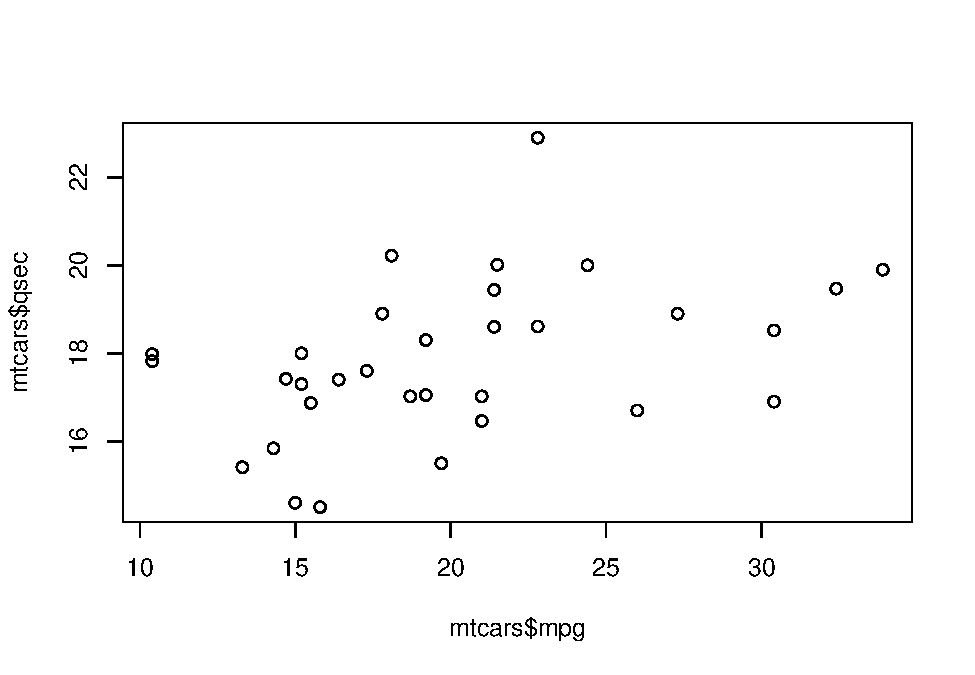
\includegraphics{Testing_files/figure-latex/NAMECODECHUNK-1.pdf}
\caption{\label{fig:NAMECODECHUNK}CHANGE FIGURE CAPTION HERE}
\end{figure}

THIS IS MY NEW FIGURE (Figure\ref{fig:NEWCODECHUNK})

\begin{figure}
\centering
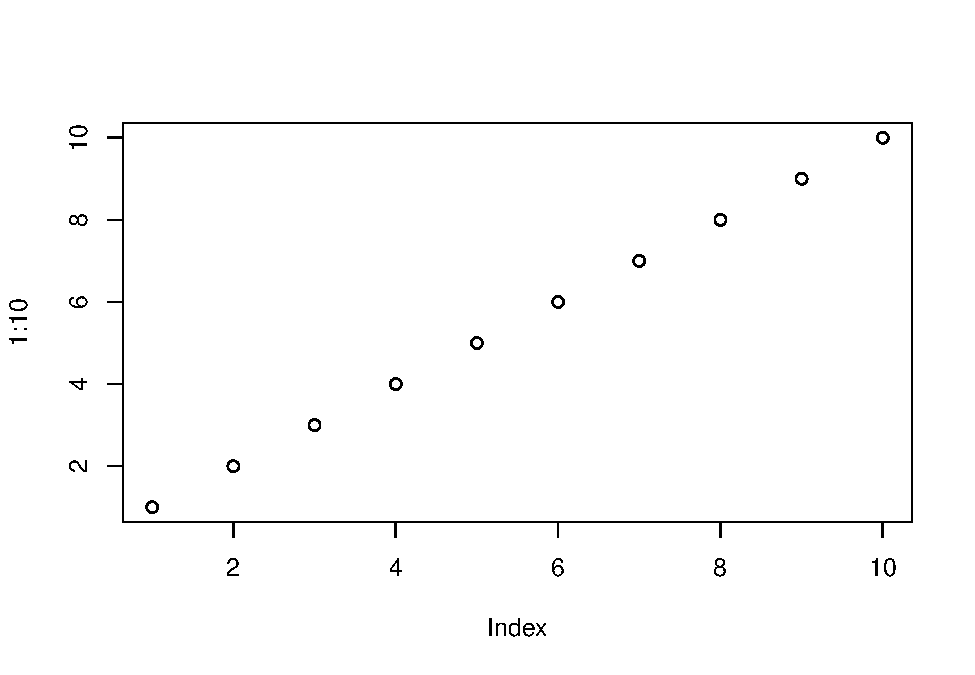
\includegraphics{Testing_files/figure-latex/NEWCODECHUNK-1.pdf}
\caption{\label{fig:NEWCODECHUNK}THI IS JUST AN EXAMPLE PLOT}
\end{figure}

\end{document}
